\section{Verifikation}
\label{sec:Verifikation}

Einfache Beispiele vorstellen, um die Programmfunktionalit�t aufzuzeigen\\

\subsection{Fallbeispiel: 2 Objekte, 1 Sensor}
\label{sec:einfFBsp}
einfache Szene: 2 Objekte + 1 Sensor, 2.72 Sekunden\\

\begin{figure}[htbp]%
\centering
{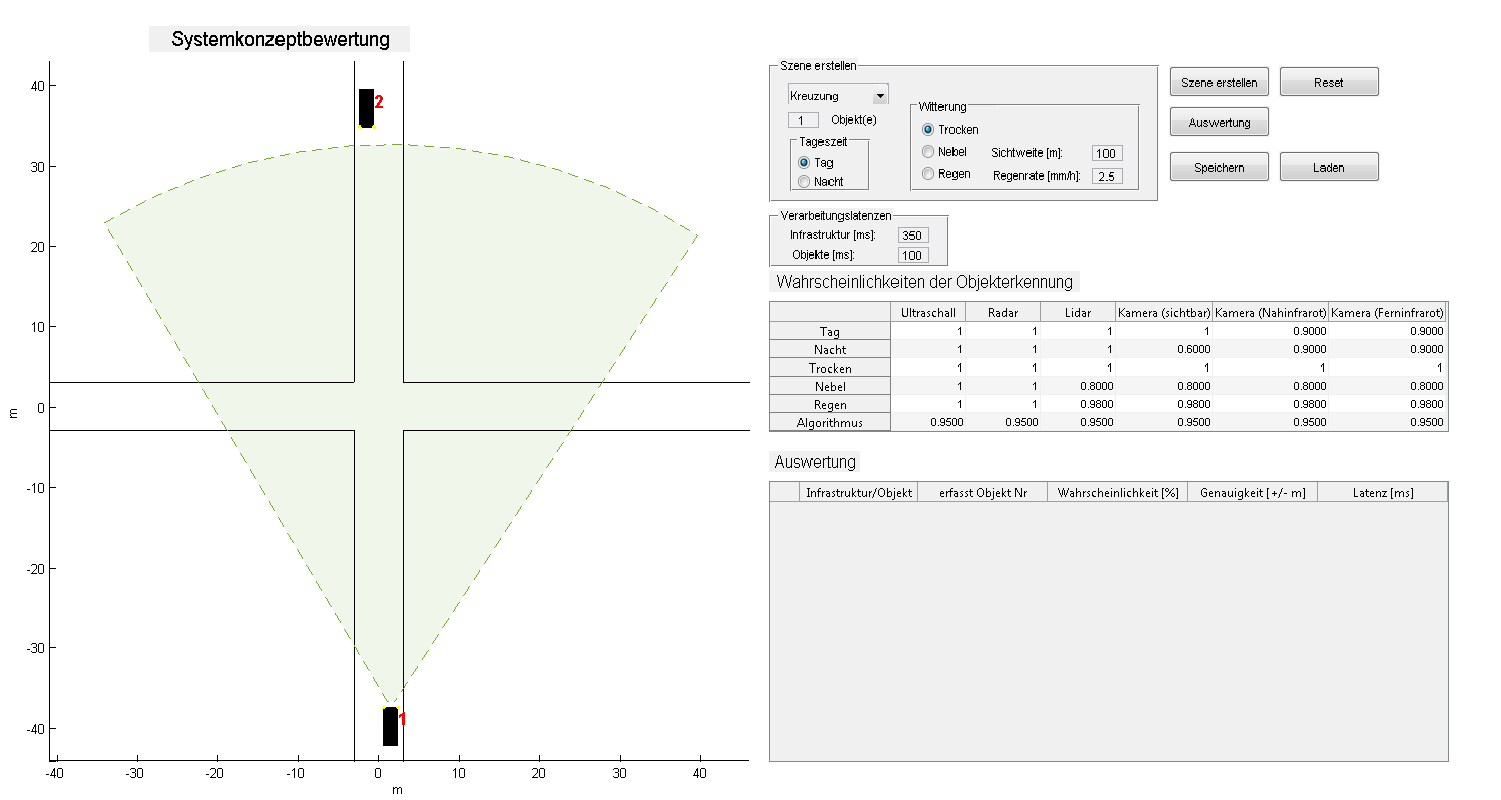
\includegraphics[width=0.8\textwidth,trim={0.2cm 0.2cm 19.9cm 2.9cm},clip]{pics/Probeszene.PNG}
\caption{Testszene: 2 Objekte, 1 Sensor bei \unit{0}{s}\label{fig:Probe}}
\end{figure}

\begin{figure}[htbp]%
\centering
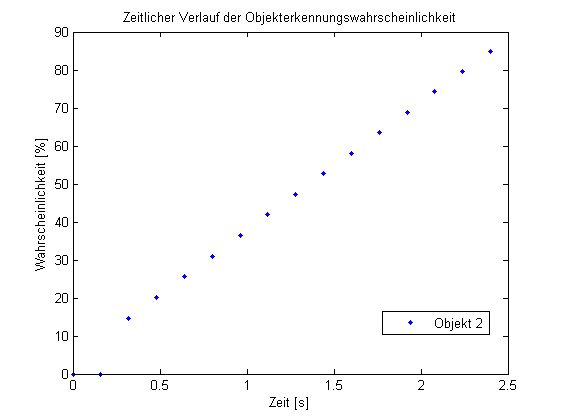
\includegraphics[width=0.7\columnwidth]{pics/fig_Probe_Wahrscheinlichkeit.png}%
\caption{Zeitlicher Verlauf der Erkennungswahrscheinlichkeit}%
\label{fig:ProbeWahr}%
\end{figure}

\subsection{Fallbeispiel: Sensoreinfl�sse}
\label{{sec:EinflFBsp}
Einfl�sse vorstellen: 1 Objekt + 1 Sensor an Infrastruktur\\
\begin{figure}[htbp]%
\centering
{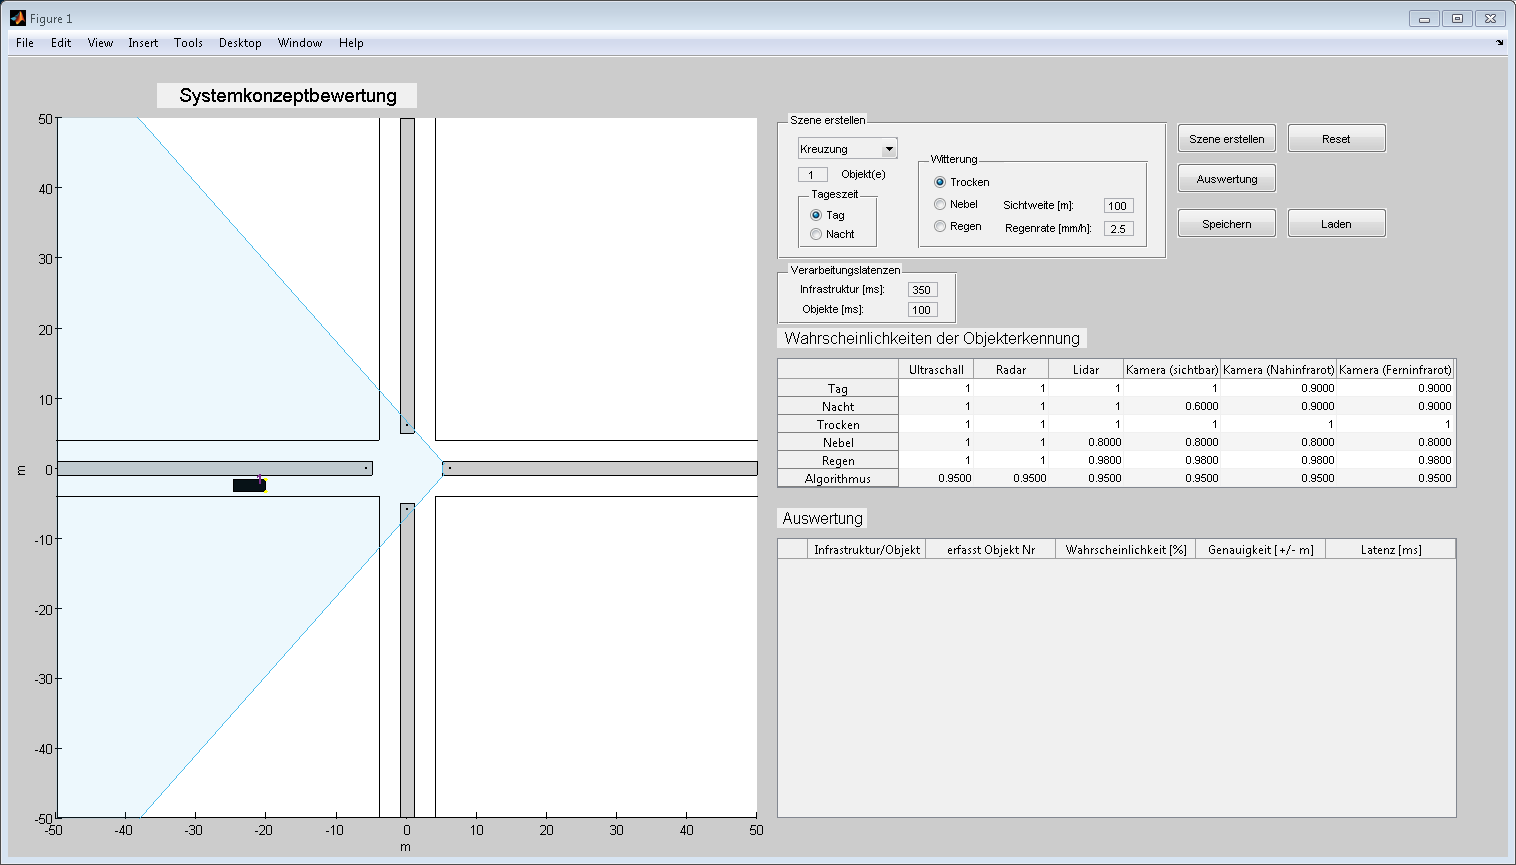
\includegraphics[width=0.8\textwidth,trim={0.2cm 0.2cm 19.9cm 2.9cm},clip]{pics/SzeneEinfluss.PNG}
\caption{Testszene: Objekt wird von einer Infrastrukturkamera erfasst\label{fig:Einfluss}}
\end{figure}
%\begin{table}
\begin{tabularx}{0.6\textwidth}{llc}%
%\centering
\caption{Einfluss der Tageszeit und Witterung bei einer Kamera im sichtbaren Spektrum}
\label{tab:Einfluss}\\\toprule%\hline
\textbf{Witterung} & \textbf{Tageszeit} & \textbf{Wahrscheinlichkeit [\%]}\\ \midrule%\hline
Trocken & Tag & 71.25	\\
Trocken & Nacht &	42.75\\
Nebel (\unit{100}{m}) & Tag & 57	\\
Regen (\unitfrac[2.5]{mm}{h}) & Tag & 68.615\\ \bottomrule%\hline
\end{tabularx}
%\end{table}
